% ME563 - HW 4
% Tyler Jones

\documentclass[11pt]{article}
\usepackage[margin=1in]{geometry}
\usepackage{amsmath, amssymb}
\usepackage{mathpazo}
\usepackage[T1]{fontenc}
\usepackage{microtype}
\usepackage{graphicx}
\usepackage{booktabs}
\usepackage{float}
\usepackage{xcolor}
\usepackage[font=small, labelfont=bf]{caption}
\usepackage{titlesec}
\usepackage{fancyhdr}
\usepackage[colorlinks=true, allcolors=blue]{hyperref}

% ---- headers / footers ------------------------------------------------
\pagestyle{fancy}
\fancyhf{}
\setlength{\headheight}{14pt}
\renewcommand{\headrulewidth}{0.4pt}
\fancyhead[L]{\small ME 563: HW 4}
\fancyhead[R]{\small Tyler Jones}
\fancyfoot[C]{\small \thepage}

% ---- section spacing --------------------------------------------------
\titleformat{\section}{\large\bfseries}{}{0pt}{}[\vspace{-0.6\baselineskip}\rule{\textwidth}{0.4pt}]
\titlespacing*{\section}{0pt}{1.6\baselineskip}{0.8\baselineskip}
\titlespacing*{\subsection}{0pt}{1.1\baselineskip}{0.4\baselineskip}

% ---- table spacing ----------------------------------------------------
\renewcommand{\arraystretch}{1.25}

% ---- shorthands -------------------------------------------------------
\newcommand{\pd}[2]{\frac{\partial #1}{\partial #2}}
\newcommand{\vect}[1]{\mathbf{#1}}

\title{\vspace{-1.5em}\textbf{ME563 HW 4}}
\author{Tyler Jones}
\date{Due: October 7, 2026}

\begin{document}
\maketitle
\thispagestyle{fancy}

%=======================================================================
\section*{Problem 1}

\noindent\textbf{Problem statement.} Incompressible fluid flows past an impermeable flat plate, with
a uniform inlet profile $u = U_0$ and a cubic polynomial exit profile
$u = U_0\,\dfrac{3\eta - \eta^3}{2}$ where $\eta = \dfrac{y}{\delta}$.

\medskip
\noindent The CV is the rectangle $0 \le y \le \delta$ between the inlet and exit, width $b$ into the
page. The flow is steady and incompressible, the bottom face is the impermeable plate, and $u = U_0$
at $y = \delta$. Reynolds transport theorem for a fixed CV, with $B$ the extensive property and
$\beta = dB/dm$:
\begin{equation*}
\frac{dB_{sys}}{dt} = \frac{d}{dt}\int_{CV}\rho\,\beta\,dV + \int_{CS}\rho\,\beta\,(\vect u\cdot\hat{\vect n})\,dA
\end{equation*}

\subsection*{(a)}

\noindent\textit{Problem statement.} Determine the volume flow $Q$ across the top surface of the
control volume.

\medskip
\noindent Mass ($\beta = 1$, $dm_{sys}/dt = 0$), steady with constant $\rho$:
\begin{equation*}
\int_{CS} \vect u\cdot\hat{\vect n}\,dA = 0
\;\Rightarrow\;
-\int_0^\delta U_0\,b\,dy + Q + \int_0^\delta u(y)\,b\,dy = 0
\end{equation*}
Exit flux, with $dy = \delta\,d\eta$:
\begin{equation*}
\int_0^\delta u\,b\,dy = U_0 b\delta\int_0^1 \frac{3\eta-\eta^3}{2}\,d\eta
= U_0 b\delta\cdot\frac12\left(\frac32 - \frac14\right) = \frac58\,U_0 b\delta
\end{equation*}
\begin{equation*}
-U_0 b\delta + Q + \frac58\,U_0 b\delta = 0
\;\Rightarrow\;
\boxed{Q = \frac38\,U_0\,b\,\delta \quad (\text{out of the CV})}
\end{equation*}
The plate slows the fluid near the wall, so $3/8$ of the inflow is displaced out through the top.

\subsection*{(b)}

\noindent\textit{Problem statement.} Determine the drag force exerted on the flow by the solid plate.
Assume pressure is uniform, and hence there's no net pressure force.

\medskip
\noindent $x$-momentum ($\beta = u$), steady. The only $x$-force on the fluid is the plate force
$F_x$:
\begin{equation*}
F_x = \int_{CS} u\,\rho\,(\vect u\cdot\hat{\vect n})\,dA
\end{equation*}
Fluid leaving through the top carries $x$-momentum $\rho U_0$ per unit volume:
\begin{align*}
\text{inlet:}&\quad -\int_0^\delta \rho U_0^2\,b\,dy = -\rho U_0^2 b\delta \\
\text{top:}&\quad \rho U_0\,Q = \frac38\,\rho U_0^2 b\delta \\
\text{exit:}&\quad \int_0^\delta \rho u^2\,b\,dy
= \rho U_0^2 b\delta\int_0^1 \left(\frac{3\eta-\eta^3}{2}\right)^2 d\eta
= \frac{\rho U_0^2 b\delta}{4}\int_0^1 \left(9\eta^2 - 6\eta^4 + \eta^6\right) d\eta \\
&\quad = \frac{\rho U_0^2 b\delta}{4}\left(3 - \frac65 + \frac17\right)
= \frac{17}{35}\,\rho U_0^2 b\delta
\end{align*}
\begin{gather*}
F_x = \rho U_0^2 b\delta\left(-1 + \frac38 + \frac{17}{35}\right)
= \rho U_0^2 b\delta\,\frac{-280 + 105 + 136}{280} \\
\boxed{F_x = -\frac{39}{280}\,\rho U_0^2\,b\,\delta \approx -0.139\,\rho U_0^2 b\delta}
\end{gather*}
The plate pulls the flow upstream ($-x$) with magnitude $\frac{39}{280}\rho U_0^2 b\delta$. By
Newton's third law, the drag on the plate is equal and opposite ($+x$).

%=======================================================================
\section*{Problem 2}

\noindent\textbf{Problem statement.} Derive a formula for the horizontal force $F$ required to hold the
gate. At sections 1 and 2, the flow is uniform. Neglecting bottom friction. Assume steady
incompressible flow with no variation across the width $b$. Express your final formula in terms of
the inlet velocity $V_1$, eliminating $V_2$.

\medskip
\noindent The CV runs from section 1 to section 2 and contains the gate. The streamlines at 1 and 2
are straight and parallel, so the pressure there is hydrostatic. Atmospheric pressure acts on the
whole CS and cancels, so I use gage pressure. $F$ is the force of the gate on the fluid, acting in
$-x$ as drawn.

\medskip
\noindent Mass:
\begin{equation*}
\rho V_1 h_1 b = \rho V_2 h_2 b
\;\Rightarrow\;
V_2 = V_1\frac{h_1}{h_2}
\end{equation*}
Hydrostatic pressure forces:
\begin{equation*}
F_{p1} = \int_0^{h_1}\rho g(h_1 - y)\,b\,dy = \frac12\rho g h_1^2 b \;(+x), \qquad
F_{p2} = \frac12\rho g h_2^2 b \;(-x)
\end{equation*}
$x$-momentum, with $\dot m = \rho V_1 h_1 b$:
\begin{equation*}
\sum F_x = \int_{CS} u\,\rho(\vect u\cdot\hat{\vect n})\,dA
\;\Rightarrow\;
\frac12\rho g b h_1^2 - \frac12\rho g b h_2^2 - F = \rho V_1 h_1 b\,(V_2 - V_1)
\end{equation*}
Substituting $V_2 - V_1 = V_1\left(h_1/h_2 - 1\right)$:
\begin{equation*}
\boxed{F = \frac12\rho g b\left(h_1^2 - h_2^2\right) - \rho b h_1 V_1^2\left(\frac{h_1}{h_2} - 1\right)}
\end{equation*}
As $V_1 \to 0$ this reduces to the net hydrostatic force. Because the flow accelerates through the
gate ($V_2 > V_1$), the momentum term lowers the force needed to hold the gate.

%=======================================================================
\section*{Problem 3}

\noindent\textbf{Problem statement.} When a uniform stream flows past an immersed thick cylinder, a
broad low-velocity wake is created downstream, idealized as a ``V''. Pressures at 1 and 2 are
approximately equal. If the flow is two-dimensional and incompressible, with width $b$ into the
paper, determine the drag force $F$ exerted on the flow by the cylinder.

\medskip
\noindent The CV is a rectangle from section 1 to section 2, with its top and bottom at $y = \pm H$
in the free stream ($H > L$). Since $p_1 \approx p_2$ and the pressure along the top and bottom is
uniform, there is no net pressure force, and shear on the top and bottom is negligible. The only
$x$-force on the fluid is $F_x$, the force of the cylinder on the flow. By symmetry, I work with the
upper half of the wake, $0 \le y \le L$:
\begin{equation*}
u(y) = \frac{U}{2}\left(1 + \frac{y}{L}\right) = \frac{U}{2}(1+\eta), \qquad \eta = \frac{y}{L}
\end{equation*}

\medskip
\noindent Mass. The wake has a velocity deficit, so a flow $Q$ leaves through the top and bottom:
\begin{align*}
Q &= \underbrace{2HU}_{\text{inlet}} - \underbrace{2(H-L)U}_{\text{exit, outside wake}}
 - \underbrace{2\int_0^L \frac{U}{2}\left(1 + \frac{y}{L}\right)dy}_{\text{exit, wake}}
 \quad(\text{per unit } b) \\
&= 2UL - UL\left(1 + \frac12\right)
\;\Rightarrow\;
Q = \frac12\,U L\,b
\end{align*}
That flow leaves in the free stream, so it carries $x$-momentum $\rho U$ per unit volume.

\medskip
\noindent $x$-momentum:
\begin{equation*}
F_x = \int_{CS} u\,\rho(\vect u\cdot\hat{\vect n})\,dA
\end{equation*}
Wake contribution:
\begin{equation*}
2\int_0^L \rho u^2\,dy = 2\rho\frac{U^2}{4}L\int_0^1 (1+\eta)^2\,d\eta
= \frac{\rho U^2 L}{2}\left[\frac{(1+\eta)^3}{3}\right]_0^1 = \frac76\,\rho U^2 L
\end{equation*}
Summing over the CS (per unit $b$):
\begin{align*}
\frac{F_x}{\rho U^2 b} &= \underbrace{-2H}_{\text{inlet}} + \underbrace{\frac12 L}_{\text{top+bottom}}
 + \underbrace{2(H - L)}_{\text{exit, outside}} + \underbrace{\frac76 L}_{\text{exit, wake}}
 = L\left(\frac12 - 2 + \frac76\right) = -\frac{L}{3}
\end{align*}
\begin{equation*}
\boxed{F_x = -\frac13\,\rho U^2\,b\,L}
\end{equation*}
$H$ drops out, as it should. The cylinder exerts a force of $\frac13\rho U^2 bL$ on the flow,
directed upstream. The drag on the cylinder is equal and opposite ($+x$).

%=======================================================================
\section*{Problem 4}

\noindent\textbf{Problem statement.} Consider water waves in a channel of depth $H$. Suppose that the
span-wise width of the channel is large and the waves are two-dimensional. The undisturbed water
level $y = 0$, is disturbed by the wave to $y = h(x,t) = A\cos(kx - \omega t)$, where $A$ denotes the
amplitude of the waves. The bottom of the channel is located at $y = -H$, and is rigid. Suppose the
velocity field due to the wave is given by:
\begin{align*}
u(x,y,t) &= -A\omega\sin(kx-\omega t)\,\cosh\!\big(k(y+H)\big)/\sinh(kH) \\
v(x,y,t) &= \phantom{-}A\omega\cos(kx-\omega t)\,\sinh\!\big(k(y+H)\big)/\sinh(kH)
\end{align*}

\medskip
\noindent Let $\theta = kx - \omega t$ and $C = A\omega/\sinh(kH)$.

\subsection*{(1)}

\noindent\textit{Problem statement.} Is this an incompressible flow?

\begin{equation*}
\pd{u}{x} = -Ck\cos\theta\,\cosh k(y+H), \qquad
\pd{v}{y} = Ck\cos\theta\,\cosh k(y+H)
\end{equation*}
\begin{equation*}
\nabla\cdot\vect u = \pd{u}{x} + \pd{v}{y} = 0
\;\Rightarrow\;
\boxed{\text{Yes, the flow is incompressible.}}
\end{equation*}

\subsection*{(2)}

\noindent\textit{Problem statement.} Compute the vorticity field associated with this flow.

\medskip
\noindent For planar flow, only $\omega_z$ is nonzero:
\begin{equation*}
\pd{v}{x} = -Ck\sin\theta\,\sinh k(y+H), \qquad
\pd{u}{y} = -Ck\sin\theta\,\sinh k(y+H)
\end{equation*}
\begin{equation*}
\omega_z = \pd{v}{x} - \pd{u}{y} = 0
\;\Rightarrow\;
\boxed{\boldsymbol\omega = \vect 0}
\end{equation*}
The flow is irrotational. It is the gradient of the potential
$\phi = -\dfrac{A\omega}{k}\sin\theta\,\dfrac{\cosh k(y+H)}{\sinh(kH)}$.

\subsection*{(3)}

\noindent\textit{Problem statement.} Find the pathlines for this flow. For this purpose take
$A/H = 10^{-3}$ and $kH = 10$ and integrate the equation numerically and show the result as a graph
of the computed pathlines. You can show the pathline originating at $x_0 = 0.5$, and $y_0 = 0.0$ at
$t = 0$. Choose suitable non-dimensional variables in your calculation and plot, please define the
choices you make.

\medskip
\noindent Pathlines satisfy $d\vect x/dt = \vect u(\vect x, t)$. I nondimensionalize length by
the depth and time by the wave frequency:
\begin{equation*}
x^* = \frac{x}{H}, \qquad y^* = \frac{y}{H}, \qquad t^* = \omega t
\end{equation*}
Since $dx/dt = \omega H\,dx^*/dt^*$, this gives
\begin{align*}
\frac{dx^*}{dt^*} &= -\frac{A}{H}\,\sin\!\big(kH\,x^* - t^*\big)\,\frac{\cosh\!\big(kH(y^*+1)\big)}{\sinh(kH)} \\
\frac{dy^*}{dt^*} &= \phantom{-}\frac{A}{H}\,\cos\!\big(kH\,x^* - t^*\big)\,\frac{\sinh\!\big(kH(y^*+1)\big)}{\sinh(kH)}
\end{align*}
The equations depend only on $A/H = 10^{-3}$ and $kH = 10$, so $k$ and $\omega$ are not needed. I
take the initial condition $(x^*_0, y^*_0) = (0.5, 0)$ at $t^* = 0$. The system was integrated over
10 wave periods ($0 \le t^* \le 20\pi$) with SciPy's \texttt{solve\_ivp} (DOP853,
$\text{rtol} = 10^{-11}$) in \texttt{hw4\_problem4.py}. Figure~\ref{fig:pathlines}(a) shows the
required pathline. Figure~\ref{fig:pathlines}(b) adds pathlines starting at three depths below the
surface, plotted as displacement scaled by $A$.

\begin{figure}[H]
  \centering
  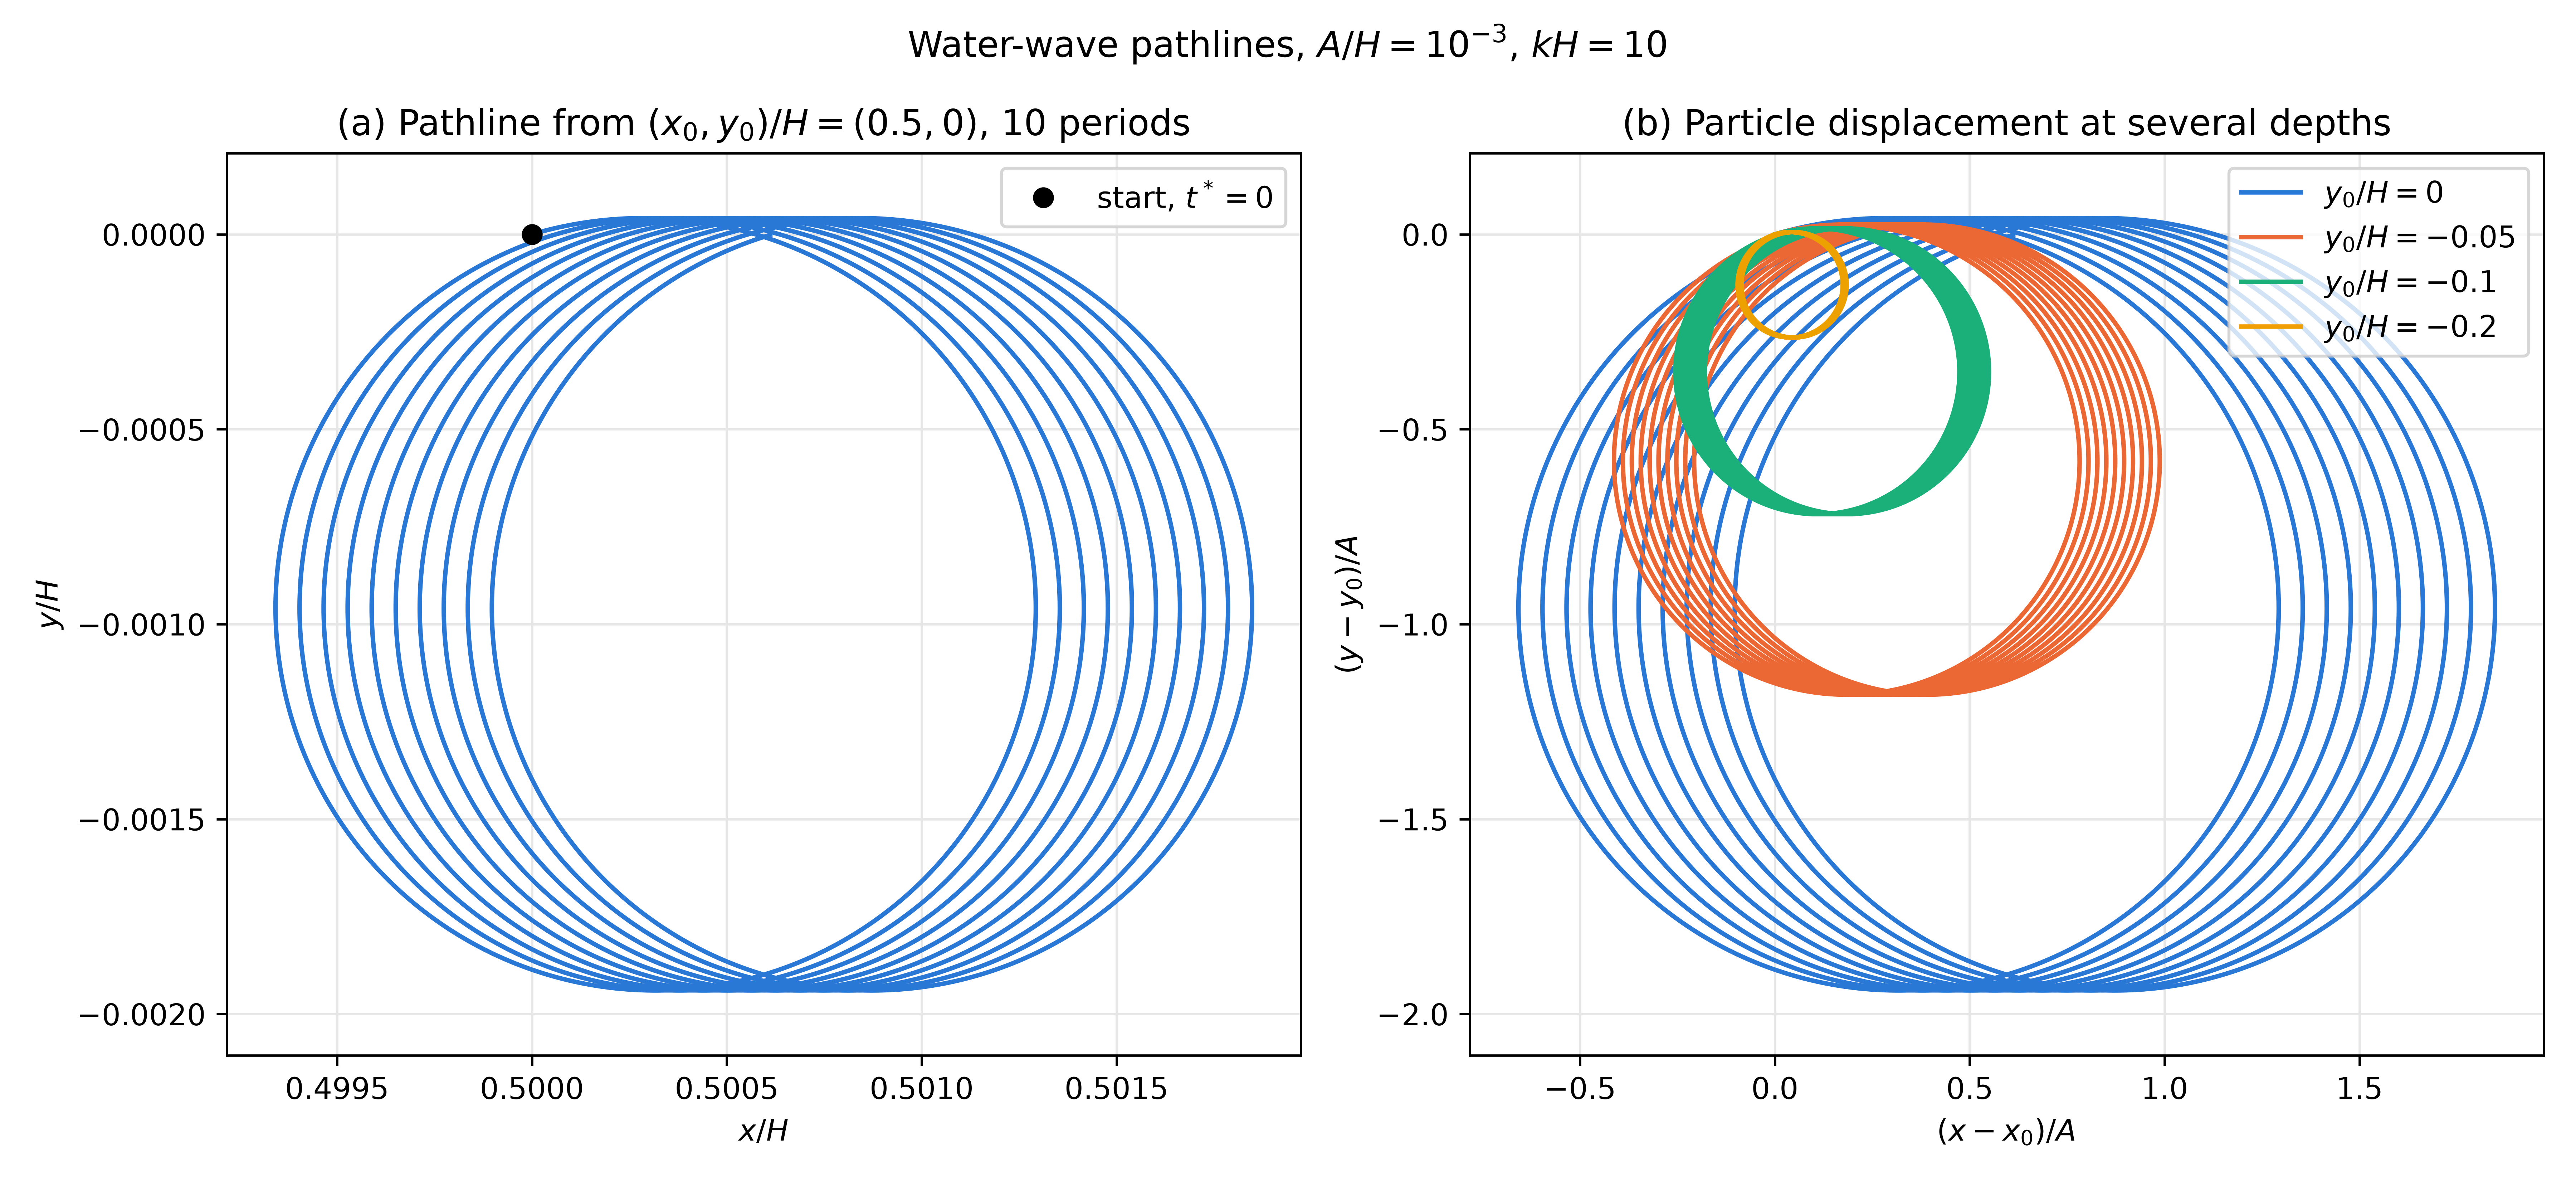
\includegraphics[width=\textwidth]{../figures/hw4_p4_pathlines.png}
  \caption{Pathlines for $A/H = 10^{-3}$, $kH = 10$ over 10 wave periods. (a) Pathline from
  $(x_0, y_0)/H = (0.5, 0)$. (b) Displacement from the starting point, scaled by $A$, for
  $y_0/H = 0,\,-0.05,\,-0.1,\,-0.2$.}
  \label{fig:pathlines}
\end{figure}

\noindent Observations:
\begin{itemize}
  \item With $kH = 10$, $\tanh(kH) \approx 1$, so this is a deep-water wave. The particles move on
  near-circular orbits of radius $\approx A\,e^{k y_0}$. The radius is about $A$ at the surface and
  decays quickly with depth, to about $0.14A$ at $y_0/H = -0.2$.
  \item The orbits do not quite close. Each period, the particle drifts forward slightly, which is
  Stokes drift, a second-order effect. The drift per period from the integration agrees with the
  Stokes result $\bar u_s = A^2\omega k\cosh\!\big(2k(y+H)\big)/\big(2\sinh^2 kH\big)$ to within
  about 3\%:
\end{itemize}
\begin{table}[H]
  \centering
  \begin{tabular}{ccc}
    \toprule
    $y_0/H$ & Drift per period$/A$ (numerical) & Drift per period$/A$ (Stokes) \\
    \midrule
    $\phantom{-}0$    & 0.0611 & 0.0628 \\
    $-0.05$           & 0.0227 & 0.0231 \\
    $-0.10$           & 0.0084 & 0.0085 \\
    $-0.20$           & 0.0011 & 0.0012 \\
    \bottomrule
  \end{tabular}
\end{table}
\noindent The flow is unsteady, so these pathlines are not the instantaneous streamlines.

\end{document}
